\subsection{USB-B}
\label{subsec:USB-B}

Auf der Leiterplatte des PartyMixer's gibt es zwei Komponenten, welche programmiert werden müssen. Der Mikrocontroller und das WiFi-Modul. Beide werden über die UART-Schnittstelle 0 programmiert. Um diese zu programmieren braucht es eine entsprechende Schnittstelle, welche mit einer USB-B-Schnittstelle realisiert wird.

Die USB-B-Schnittstelle benötigt jedoch nur zwei Kommunikationsleitungen (D+ und D-). Deswegen benötigt es einen USB-UART-Converter. Hier wurde auf das Flash-Interface von Arduino zurückgegriffen \cite{arduino_cc_arduino_2017}, um die Schaltung für den Mikrocontroller zu planen und auf das Flash-Interface des ESP32 \cite{espressif_systems_esp32_2016}, um die Schaltung für den ESP32 zu planen. Darin ist ersichtlich, dass für den Mikrocontroller und ESP folgende Leitungen nötig sind:

\begin{itemize}
\item Mikrocontroller
\begin{itemize}
\item RX ==> TX
\item TX ==> RX
\item Reset ==> über Kondensator an DTR
\end{itemize}
\item ESP32
\begin{itemize}
\item RX ==> TX
\item TX ==> RX
\item EN ==> über Schaltung an DTR
\item IO\_0 ==> über Schaltung an RTS
\item IO\_13 ==> über Widerstand an RTS
\item IO\_15 ==> über Widerstand an CTS
\end{itemize}
\end{itemize}

Auch hier wurde vom Arduino Uno-Board abgekpufert und der selbe Chip verwendet, um die USB-Signale in UART-Signale zu konvertieren. Das vorkommende Bauteil ist der CP2102N. Da dieser Chip ein TQFP-28-Gehause hat, könnte es auch schwierigkeiten geben beim Löten. Deswegen wird auch ein Breakout-Board (BOB) mitgeplant, damit es eine Ausweichmöglickeit gibt falls die Bauteile zu klein sind. Dabei ist zu achten, dass das BOB genügend Ausgangspins hat, speziell beim ESP32.

\begin{figure}[!h]
\center
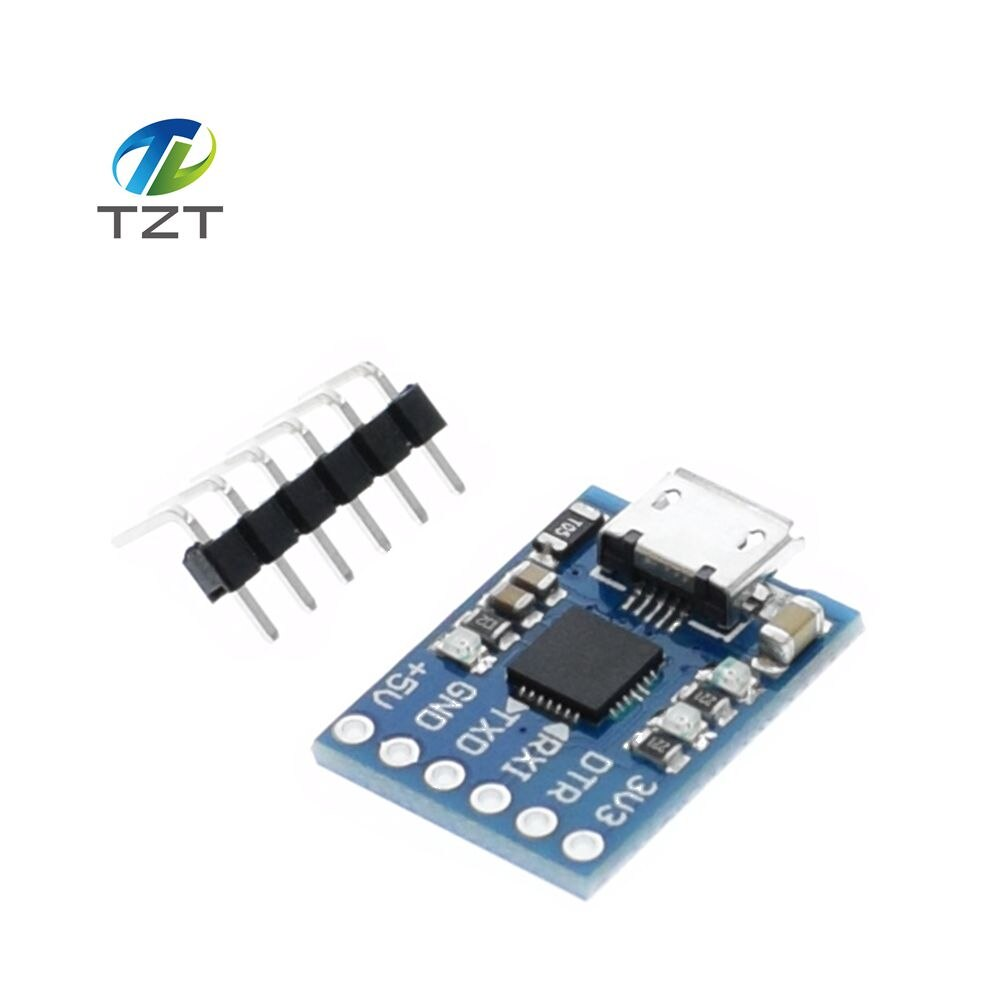
\includegraphics[width = 0.5\textwidth]{graphics/Produktbild_USB_UART_uC}
\caption{CP2102N-BOB für uC.}
\label{fig:Produktbild_USB_UART_uC}
\end{figure}

\begin{figure}[!h]
\center
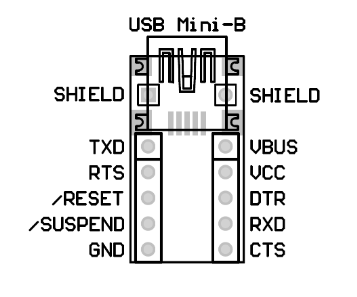
\includegraphics[width = 0.5\textwidth]{graphics/Produktbild_USB_UART_ESP}
\caption{CP2102N-BOB für ESP.}
\label{fig:Produktbild_USB_UART_ESP}
\end{figure}